\chapter{USB}
El \emph{Universal Serial Bus}(USB\footnote{V\'ease - http://www.usb.org}) es
un bus serial ent\'andar que hace de interfaz entre un dispositivo y una
computadora.
Dicha estandarizaci\'on es llevada acabo por el \emph{F\'orum de
Implementadores de USB} (USB Implementers Forum, USB-IF\footnote{V\'ease -
http://www.usb.org/about}). 
Actualmente el est\'andar se encuentra en su versi\'on 3.0\footnote{V\'ease -
http://www.usb.org/developers/docs/}, aunque la mayor\'ia de las
implementaciones comerciales solo soportan el ent\'andar \emph{2.0}.

\section{Historia}
%No me gusta como titulo 'historia' habria que pensar otra cosa

\section{Decripci\'on}
% Aca iria el funcionamiento del USB, difierenciado por \subsection{}
% Por ahora me estoy basando en la spec 2.0 oficial.
La especificaci\'on USB provee una serie de atributos con los cuales se pueden
implementar dispositivos seg\'un el precio/rendimiento deseado.

\subsection{Caracter\'isticas}
Del amplio rango de caracter\'isticas definidas en el ent\'andar, es posible
agruparlas en ocho categor\'ias:
% Reescribir lo de arriba y agregar mas

\begin{itemize}
 \item Facilidad de uso para el usuario final
 \item Amplio rango de aplicaciones
 \item Ancho de banda is\'ocrono
 \item Flexibilidad
 \item Robustez
 \item Sinergia con la industria de la PC
 \item Implementaci\'on de bajo costo
 \item De arquitectura actualizable
\end{itemize}

La combinaci\'on de estas caracter\'isticas hacen a la versatilidad del
ent\'andar, ya que permiten implementar todo tipo de dispositivos seg\'un la
carga, versatilidad, eficiencia, precio, velocidad y dem\'as atributos que
puedan inferir en un diese\~no.\\

Para la veri\'on 2.0 de la epecificaci\'on, el protocolo soporta tres
velocidades de transimsi\'on como se muestra en la
tabla \ref{tab:velocidad_usb}.

\begin{table}[h]
\centering
% use packages: array,booktabs
\begin{tabular}{|c|c|}        \hline
High Speed & 480 Mbits/seg \\ \hline 
Full Speed & 12 Mbits/seg  \\ \hline
Low Speed & 1.5 Mbits/seg  \\ \hline
\end{tabular}
\caption{Velocidades de USB} 
\label{tab:velocidad_usb}
\end{table}

\subsection{Arquitectura}

USB es un \emph{bus} cableado que soporta conexiones entre un \emph{host} y
gran rango de perif\'ericos. Dicho \emph{bus} permite la conexi\'on,
configuraci\'on, uso y desconexi\'on de un dispositivo mientras el \emph{host}
y dem\'as perif\'ericos est\'an en funcionamiento. \\

Un sistema USB se  define segun tres grandes \'areas:

\begin{itemize}
 \item Interconexi\'on USB
 \item Dispositivo USB
 \item \emph{Host} USB
\end{itemize}

\subsubsection{Caracter\'isticas el\'ectricas}

USB usa cuatro cables para alimentaci\'on y se\~nal. La se\~nal viaja a travez
de un par trenzado diferencial y se encuentra codificada con Non Return to Zero
Inverted (NRZI). En la figura \ref{fig:electric_usb} se muestra un diagrama de
un cable
USB.

\begin{figure}
\centering
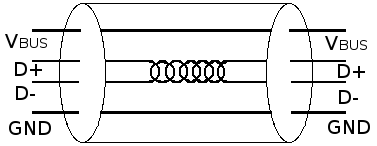
\includegraphics[scale=0.5]{./img/electric_usb.png}
\caption{Cable USB.}
\label{fig:electric_usb}
\end{figure}

Al ser un par diferencial, el host iterpreta un \emph{1} diferencial cuando D+
es 200 mV mayor que D- y un \emph{0} diferencial cuando D- es 200 mV mayor que
D+. 
Los dispositivos USB indican su velocidad mediante una resistencia de
\emph{pull-up} a 3.3 V. En el caso de un \emph{full speed device} se col\'oca
una resistencia de 1.5K en D+ a 3.3 V, y para \emph{low speed device} se coloca
una resistencia de 1.5K a 3.3 V, como se muestra en la figura
\ref{fig:electric_speed_usb}.
Algunos fabricantes sulen integrar estas resistencias de \emph{pull-up} dentro
de sus \emph{chips} para ser activadas mediante software.

\begin{figure}
\centering
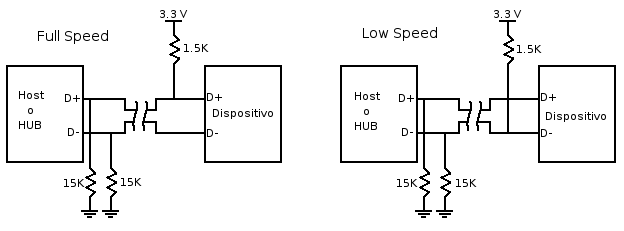
\includegraphics[scale=0.5]{./img/electric_speed_usb.png}
\caption{Velocidad USB.}
\label{fig:electric_speed_usb}
\end{figure}


\subsection{Interconexi\'on USB}

La interconexi\'on USB define la manera en la que los dispositivos USB se
conectan entre si y con el \emph{host}. 

\subsubsection{Topolog\'ia del bus}

USB usa una topolog\'ia de estrella por niveles. Un \emph{hub}\footnote{La
palabra \emph{hub} se traduce al castellano como \emph{centro}, pero su
traducci\'on no sera usada en este documento por cuestiones pr\'acticas.}
est\'a ubicado al centro de cada estrella. Las conexiones cableadas se dan
entre el \emph{host} y un \emph{hub} o funci\'on, entre \emph{hub} y
\emph{hub}, o entre un \emph{hub} y una funci\'on. \\

Debido a cuestiones de latencia, el n\'umero m\'aximo de niveles permitido es
siete, incluida la ra\'iz. La figura \ref{fig:usb_topology} muestra un esquema
de la topolog\'ia.

\begin{figure}
\centering
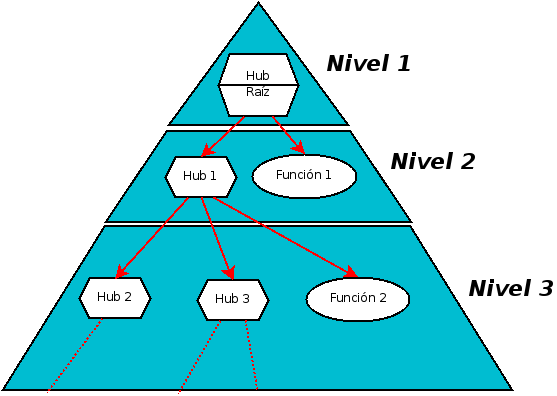
\includegraphics[scale=0.5]{./img/usb_topology.png}
\caption{Topolog\'ia del bus USB.}
\label{fig:usb_topology}
\end{figure}

\subsection{\emph{Host} USB}

La especificaci\'on admite un solo \emph{Host} para un todo sistema USB. La
interf\'az USB del \emph{host}, se la denomina \emph{Host
Controller}\footnote{Al igual que con \emph{host}, esta palabra se mantedr\'a
en ingles.}. La implementaci\'on de un \emph{Host Controller} puede ser una
combinaci\'on de hardware, firmware o software. El \emph{hub} ra\'iz esta
integrado en el sistema \emph{host}, proveyendo puntos de acceso.
En la versi\'on 1.1 de la especificaci\'on, exixtian dos tipod de
controladores de \emph{hots}; \emph{Universal Host Controller Interface}
(UHCI)\footnote{Desarrolada por Intel} y \emph{Open Host Controller Interface}
(OHCI)\footnote{Desarrollada por Compaq, Microsoft y National Semiconductors}.
Luego con para le versi\'on 2.0 de la especificaci\'on de defini\'o un tercer
controlador; \emph{Enhanced Host Controller Interface} (EHCI)\footnote{Que
luego pasaria a convertirse en el estandar mas usado.}

\subsection{Dispositivo USB}

Los dispositivos USB pueden ser dispositivos funcionales o bien \emph{hubs}.
En ambos casos deben ser capaces de entender el protocolo USB y responder a
peticiones estandares USB ademas de cumplir su funci\'on intr\'inseca. 

% Explicar --- UHCI, OHCI, EHCI
%\begin{Huge} TERMINAR!!! \end{Huge}


El protocolo USB define capas de abstracci\'on, cada cual con una funcionalidad
espec\'ifica. Normalmente los \emph{chips} manejan las capas mas bajas, para
abstraer al usuario de todo lo que ocurre en lo mas bajo del protocolo.\\

Una transacci\'on USB consiste de los siguientes paquetes:
\begin{itemize}
 \item Token (paquete cabecera)
 \item Data (opcional)
 \item Status (handshaking)
\end{itemize}

Los paquetes USB tienen ciertos campos comunes: 
\begin{itemize}
 \item Sync: Es un campo de sincronismo y todos los paquetes deben comenzar
con uno.
 \item PID: Es el identificador de paquete que informa el tipo de paquete que
es.
 \item ADDR: Es la direcci\'on a la cual esta asignado el paquete
 \item ENDP: Este campo de 4 bits permite direccionar hasta 16
\emph{endpoints}.
 \item CRC: Lleva la informaci\'on de un chequeo de redundancia c\'iclica de
los datos
 \item EOP: Este campo indica la finalizaci\'on del paquete.
\end{itemize}


\subsubsection{Paquete \emph{Token}}
Los paquetes \emph{token} son usados para indicar el tipo de transacci\'on que
se realizar\'a. Existen tres tipos de paquetes \emph{token}:

\begin{itemize}
 \item IN - Informa al dispositivo USB que el host desea leer informaci\'on
 \item OUT - Inrofma al dispositivo USB que el host desea escribir
informaci\'on
 \item Setup - Es usado para comenzar transferencias de control
\end{itemize}

Un paquete \emph{token} esta formado por los siguientes campos mostrados en la
tabla \ref{tab:usb_token_fields}


\begin{table}[h]
\centering
% use packages: array,booktabs
\begin{tabular}{|c|c|c|c|c|c|} \hline
Sync & PID & ADDR & ENDP & CRC5 & EOP\\ \hline
\end{tabular}
\caption{Campos Token} 
\label{tab:usb_token_fields}
\end{table}

\subsubsection{Paquete \emph{Data}}
Un paquete \emph{data} esta formado por los siguientes campos mostrados en la
tabla \ref{tab:usb_data_fields}

\begin{table}[h]
\centering
% use packages: array,booktabs
\begin{tabular}{|c|c|c|c|c|} \hline
Sync & PID & DATA & CRC16 & EOP\\ \hline
\end{tabular}
\caption{Campos Data} 
\label{tab:usb_data_fields}
\end{table}

\subsubsection{Paquete \emph{Status}}
Los paquetes \emph{status} son usados para indicar el tipo de estado de la
transacci\'on. Existen tres tipos de paquetes \emph{status}:

\begin{itemize}
 \item ACK - Reconocimiento de que el paquete fue recibido.
 \item NAK - Avisa de que el dispositivo no puede recibir ni enviar datos.
 \item STALL - Significa que el dispositivo necesita la intevenci\'on del host.
\end{itemize}

Un paquete \emph{status} esta formado por los siguientes campos mostrados en la
tabla \ref{tab:usb_status_fields}.

\begin{table}[h]
\centering
% use packages: array,booktabs
\begin{tabular}{|c|c|c|} \hline
Sync & PID & EOP\\ \hline
\end{tabular}
\caption{Campos Status} 
\label{tab:usb_status_fields}
\end{table}



\section{USB en linux}

Linux comenz\'o a soportar el protocolo USB desde la versi\'on 2.2.7
(\emph{principio de 1999}), con codigo aportado por el mismo \emph{Linus
Torvalds\footnote{Codigo fuente
en: ftp://ftp.kernel.org/pub/linux/kernel/testing/old/usb/}
\footnote{V\'ease:
http://marc.info/?l=linux-usb\&m=92282561930486\&w=2}
}.\\

Con el paso del tiempo el soporte de linux para el protoco USB ha aumentado
considerablemente, y actualmente existen drivers para una enorme cantidad de
dispositivos.\\

Linux interpone varias capas de abstracci\'on entre el usuario y el hardware
USB, en la figura \ref{fig:usb_linux_layers} se puede apreciar una
representacion de dichas capas.

\begin{figure}
\centering
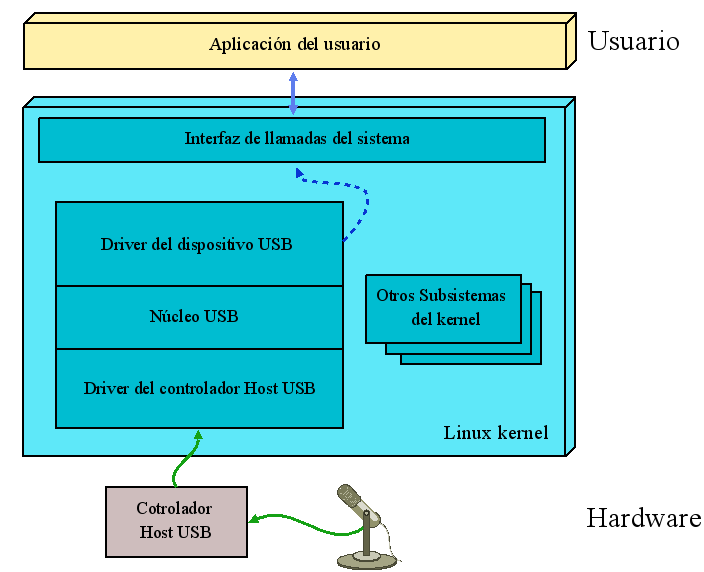
\includegraphics[scale=0.5]{./img/usb_linux_layers.png}
\caption{Soporte USB de linux.}
\label{fig:usb_linux_layers}
\end{figure}


En los cap\'itulos siguientes se describir\'a como es
manejado el protocolo a nivel del kernel y una \emph{API} libre de mas alto
nivel.

\subsection{Manejo USB de bajo nivel}

El kernel linux posee documentaci\'on embebida, la cual puede ser generada en
formato \emph{postscipt} \footnote{V\'ease -
http://es.wikipedia.org/wiki/PostScript}, pdf, o html. Para lograr esto basta
con bajar el codigo del kernel y compilar la documentaci\'on de la siguiente
manera:

\begin{scriptsize}
	\begin{verbatim}
	$ wget http://www.kernel.org/pub/linux/kernel/v2.6/linux-x.y.z.tar.bz2
	$ tar -xjf linux-x.y.z.tar.bz2
	$ cd  linux-x.y.z/
	$ make pdfdocs
	\end{verbatim}
\end{scriptsize}

En la documentaci\'on generada se encuentra una secci\'on espec\'ifica sobre
USB.\\

Basicamente linux posee en su nivel m\'as bajo drivers para el controlador
host (ya sean UHCI, OHCI o EHCI), el cual se comunica con el
\emph{usbcore}\footnote{Tambi\'en llamado API, pero aqui nos referiremos como
\emph{usbcore} o \emph{core} por cuestiones pr\'acticas.} quien interactua
directamente con los drivers espec\'ificos de cada dispositivo (Ver figura
\ref{fig:usb_linux_layers}).


%% Esto ya no es tan bajo nivel, deberi tener otra seccion
En el c\'odigo fuente del kernel existe un \emph{esquelto}\footnote{V\'ease
- http://lxr.linux.no/linux+v2.6.28/drivers/usb/usb-skeleton.c} de un driver
gen\'erico, con varias variables definidas, funciones y macros \'utiles.
Este \emph{esqueleto} fue escrito por Greg Kroah-Hartman\footnote{Mail - 
greg@kroah.com} y basado en \emph{pci-skeleton.c}\footnote{V\'ease -
http://lxr.linux.no/linux+v2.6.28/drivers/net/pci-skeleton.c}.
Este \emph{driver gen\'erico} posee todo lo necesario para , con
modificaciones suficientes, escribir un driver espec\'ifico de un dispositivo.

\subsection{URBs (API de bajo nivel)}

El kernel maneja\footnote{Si bien es la forma mas recomendada, puede evitarse
el uso de esta API} el acceso de los distintos drivers al sistema USB mediante
mensajes de \emph{pedidos de bloques USB} (\emph{URB - USB Request
Block}\footnote{El acronimo \emph{URB} se usar\'a en el documento por
cuestiones pr\'acticas}).\\

El concepto b\'asico de \emph{URBs} es el paso de mensajes de forma
asincr\'onica. 
Un \emph{URB} contine toda la informacion necesaria para hacer una
transacci\'on USB y provee ademas un \emph{manejador}\footnote{\emph{Handler}
en ingles.} con toda la informaci\'on de la transacci\'on.
Por la naturaleza as\'incrona de los URBs, ni bien se env\'ian, estos son
encolados y la funci\'on vuelve inmediatamente. 

% FAAAAKKKKK como mierda me las arreglo para explicar todo esto, que
% quilombo!!!!
% Seguir...


\subsection{API de alto nivel - libusb}

La API \emph{libusb} consiste en un set de librerias de codigo abierto
licenciadas bajo LGPL (%Expandir el nombre y poner footnote con url
% Hacer lo mismo con libusb ). 
Dichas librerias resuelven la comunicaci\'on
USB pero a nivel de usuario.
La API se encuentra en casi todoas las distribuciones de GNU/Linux, y se
presenta en forma de libreria dinamica para usar con aplicaciones ya
compiladas y un paquete extra para \emph{development}\footnote{Del ingles
desarrollo}, con los archivos cabecera, programas para compilar, y
la documentaci\'on completa de sus funcionalidades con algunos ejemplos
extras. \\

La libreria provee entre definiciones y estructuras, las siguientes funciones:
\begin{footnotesize}
\begin{verbatim}
/* usb.c */
usb_dev_handle *usb_open(struct usb_device *dev);
int usb_close(usb_dev_handle *dev);
int usb_get_string(usb_dev_handle *dev, int index, int langid, char *buf,
        size_t buflen);
int usb_get_string_simple(usb_dev_handle *dev, int index, char *buf,
        size_t buflen);

/* descriptors.c */
int usb_get_descriptor_by_endpoint(usb_dev_handle *udev, int ep,
        unsigned char type, unsigned char index, void *buf, int size);
int usb_get_descriptor(usb_dev_handle *udev, unsigned char type,
        unsigned char index, void *buf, int size);

/* <arch>.c */
int usb_bulk_write(usb_dev_handle *dev, int ep, const char *bytes, int size,
        int timeout);
int usb_bulk_read(usb_dev_handle *dev, int ep, char *bytes, int size,
        int timeout);
int usb_interrupt_write(usb_dev_handle *dev, int ep, const char *bytes, int
		size, int timeout);
int usb_interrupt_read(usb_dev_handle *dev, int ep, char *bytes, int size,
        int timeout);
int usb_control_msg(usb_dev_handle *dev, int requesttype, int request,
        int value, int index, char *bytes, int size, int timeout);
int usb_set_configuration(usb_dev_handle *dev, int configuration);
int usb_claim_interface(usb_dev_handle *dev, int interface);
int usb_release_interface(usb_dev_handle *dev, int interface);
int usb_set_altinterface(usb_dev_handle *dev, int alternate);
int usb_resetep(usb_dev_handle *dev, unsigned int ep);
int usb_clear_halt(usb_dev_handle *dev, unsigned int ep);
int usb_reset(usb_dev_handle *dev);
\end{verbatim}
\end{footnotesize}

Todas las funciones de esta libreria (para la version estable 0.1) son
s\'incronas, lo que significa que se debe esperar a que termine la operaci\'on
para poder seguir. Por este motivo la mayoria de las funciones implemetan un
\emph{timeout} en milisegundos.\\

% Poner primero, antes del codigo, un diagrama de flujo del mismo


Para comenzar una comunicaci\'on USB con esta libreria es preciso primero
descubrir el dipositivo, esto se logra con:

\begin{footnotesize}
	\begin{verbatim}
struct usb_bus *busses;
    
usb_init();
usb_find_busses();
usb_find_devices();
    
busses = usb_get_busses();
	\end{verbatim}
\end{footnotesize}

Luego de esto ya se poseen los \emph{busses} USB del sitema. Es preciso luego
iterar sobre cada uno de ellos para encontrar el dispositivo especifico de la
siguiente manera:

\begin{footnotesize}
\begin{verbatim}
struct usb_bus *bus;
int c, i, a;
    
/* ... */
    
for (bus = busses; bus; bus = bus->next) {
  struct usb_device *dev;
    
    for (dev = bus->devices; dev; dev = dev->next) {
        /* Buscar el dispositivo por VendorID */
        if (dev->descriptor.idVendor == MY_ID) {
            /* Buscar el dispositivo por ProductID */
            if (dev->descriptor.idProduct==USBPRINTER){
            /* Abrir dispositivo */
            udev = usb_open(dev);
            /* Reclamar la interfaz */
            ret = usb_claim_interface(udev,0); 

            /* Programa */
            }	...
        }
    }
}
\end{verbatim}
\end{footnotesize}

Una limitaci\'on intr\'inseca de la libreria es que se requiere abrir tantas
instancias del dispositivo como interfaces se desee usar de \'el.\\

Estas librerias satisfacen tanto el estandar USB 1.0 como el 2.0, es por ello
que si el dispositivo respeta el estandar, establecer una comunicaci\'on a
USB requiere solo la adici\'on de algunas funciones al codigo fuente para;
inicializar la comunicaci\'on, para buscar el dispositivo, para abrirlo y
luego el programa en si.

